\chapter{Bioinformatika dan Analisis Urutan}\label{ch:b3:bioinformatics}

Seorang ahli biologi yang baru saja mengurutkan sebuah gen dari cacing laut
dalam menempelkan \num{300} asam aminonya ke sebuah formulir daring dan, tiga
detik kemudian, mengetahui bahwa proteinnya adalah sepupu jauh sebuah kinase
manusia, dengan \qty{31}{\%} keidentikan sepanjang \num{280} residu dan
peluang $10^{-40}$ bahwa kemiripan itu kebetulan. Di balik ketiga detik itu
terdapat algoritma \omterm{thm:b3:bioinformatics:nw}{pemrograman dinamis} dari tahun 1970, teori statistika
\omterm{def:b3:bioinformatics:alignment}{penjajaran} acak, \omterm{def:b3:bioinformatics:matrices}{matriks substitusi} yang disaring dari ribuan famili protein,
dan sebuah pangkalan data berisi sekitar seratus miliar residu. Bab ini
membahas penalaran di dalam kotak itu: bagaimana dua urutan dijajarkan
sehingga \omterm{def:b3:bioinformatics:alignment}{penjajarannya} terbukti yang terbaik, bagaimana skornya dibuat
bermakna, bagaimana kecocokan dibedakan dari kebetulan, dan bagaimana pola
ditemukan di dalam genom yang belum pernah dilihat siapa pun. Matematikanya
sederhana --- sebuah rekurensi, sebuah logaritma, sebuah sebaran Poisson ---
dan layak diketahui, karena setiap kesimpulan yang ditarik dari perbandingan
urutan bertumpu padanya.

\section{Menjajarkan dua urutan}

\begin{definition}[Penjajaran dan skor]\label{def:b3:bioinformatics:alignment}
\index{penjajaran urutan}\index{denda celah}%
\index{penjajaran global}\index{penjajaran lokal}
Sebuah \emph{penjajaran} dua urutan menuliskan keduanya bersusun, dengan
\emph{celah} (--) yang disisipkan sehingga tiap lajurnya memasangkan satu
residu dengan satu residu atau satu residu dengan sebuah celah, dan tak ada
lajur yang memasangkan dua celah. \emph{Skornya} adalah jumlah atas lajurnya
berupa skor substitusi $s(a,b)$ bagi tiap pasangan residu ditambah sebuah
\emph{denda celah} bagi tiap celah: denda linear $-d$ tiap kedudukan celah,
atau, secara lebih masuk akal, denda \emph{afin} $-d - (k-1)e$ bagi deretan
$k$ celah, dengan ongkos pembukaan $d$ lebih besar daripada ongkos perpanjangan
$e$, karena satu sisipan berisi beberapa residu merupakan satu peristiwa
evolusi tunggal. Sebuah penjajaran \emph{global} meliputi kedua urutannya
dari ujung ke ujung; sebuah penjajaran \emph{lokal} mencari pasangan
subuntai berskor tertinggi lalu mengabaikan sisanya, dan itulah yang
diinginkan ketika sebuah domain bersama duduk di dalam dua protein yang
selebihnya tak berkerabat.
\end{definition}

\begin{theorem}[Needleman--Wunsch]\label{thm:b3:bioinformatics:nw}
\index{Needleman--Wunsch}\index{pemrograman dinamis}\index{Smith--Waterman}
Misalkan $x = x_{1}\dots x_{m}$ dan $y = y_{1}\dots y_{n}$, dengan \omterm{def:b3:bioinformatics:alignment}{denda
celah} linear $d$. Definisikan $F(i,j)$ sebagai skor terbaik \omterm{def:b3:bioinformatics:alignment}{penjajaran global}
kedua awalan $x_{1}\dots x_{i}$ dan $y_{1}\dots y_{j}$. Maka
$F(i,0) = -id$, $F(0,j) = -jd$, dan untuk $i,j \ge 1$
\[
F(i,j) = \max\bigl\{\,F(i-1,j-1) + s(x_{i},y_{j}),\;
F(i-1,j) - d,\; F(i,j-1) - d\,\bigr\}.
\]
$F(m,n)$ adalah skor global optimumnya, \omterm{def:b3:bioinformatics:alignment}{penjajaran} optimumnya dipulihkan
dengan menelusuri balik dari $(m,n)$ pilihan yang menghasilkan tiap
maksimumnya, dan seluruh perhitungannya memakan $mn$ langkah. Varian
\emph{Smith--Waterman} bagi \omterm{def:b3:bioinformatics:alignment}{penjajaran lokal} menambahkan $0$ sebagai pilihan
keempat di dalam maksimumnya, menetapkan batasnya menjadi $0$, lalu membaca
jawabannya pada entri terbesar tabelnya.
\end{theorem}
\begin{proof}
Tinjaulah lajur terakhir \omterm{def:b3:bioinformatics:alignment}{penjajaran} mana pun atas kedua awalan itu. Lajur itu
salah satu dari tiga hal: $x_{i}$ di atas $y_{j}$, $x_{i}$ di atas sebuah
celah, atau sebuah celah di atas $y_{j}$. Membuangnya meninggalkan \omterm{def:b3:bioinformatics:alignment}{penjajaran}
$(x_{1}\dots x_{i-1},
y_{1}\dots y_{j-1})$, atau $(x_{1}\dots x_{i-1}, y_{1}\dots y_{j})$, atau
$(x_{1}\dots x_{i}, y_{1}\dots y_{j-1})$, yang skornya paling banyak sebesar
$F$ pasangan itu; dan sebaliknya tiap \omterm{def:b3:bioinformatics:alignment}{penjajaran} optimum tersebut
dapat diperpanjang dengan lajur terakhir yang bersesuaian. Jadi skor terbaik
yang berakhir pada tiap macam lajur adalah $F$ pasangan yang lebih pendek
ditambah skor lajurnya, dan optimumnya adalah yang terbesar di antara
ketiganya. Batasnya terpaksa demikian (hanya celah yang mungkin berhadapan
dengan awalan kosong). Induksi atas $i + j$ mengisi tabelnya; cacah selnya
$(m+1)(n+1)$. Bagi \omterm{def:b3:bioinformatics:alignment}{penjajaran lokal}, pilihan tambahan $0$ berarti ``mulailah
\omterm{def:b3:bioinformatics:alignment}{penjajaran} baru di sini'', yang menjadikan $F(i,j)$ skor terbaik \omterm{def:b3:bioinformatics:alignment}{penjajaran}
yang \emph{berakhir} di $(i,j)$, dan \omterm{def:b3:bioinformatics:alignment}{penjajaran lokal} terbaik berakhir di suatu tempat.
\end{proof}

\begin{example}[Sebuah tabel empat kali tiga]\label{ex:b3:bioinformatics:nw-example}
Jajarkan GAT dengan GCAT, dengan skor $+1$ bagi kecocokan, $-1$ bagi
ketakcocokan, dan $d = 1$. Batasnya $0, -1, -2, -3, -4$ sepanjang atas dan
$0, -1,
-2, -3$ sepanjang sisinya. Mengisi baris demi baris: $F(\text{G},\text{G}) = 1$,
$F(\text{G},\text{C}) = 0$, $F(\text{G},\text{A}) = -1$,
$F(\text{G},\text{T}) = -2$; $F(\text{A},\text{G}) = 0$,
$F(\text{A},\text{C}) = 0$, $F(\text{A},\text{A}) = 1$,
$F(\text{A},\text{T}) = 0$; $F(\text{T},\text{G}) = -1$,
$F(\text{T},\text{C}) = -1$, $F(\text{T},\text{A}) = 0$,
$F(\text{T},\text{T}) = 2$. Optimumnya $2$, dan \omterm{met:b3:bioinformatics:align}{penelusuran baliknya}
--- diagonal dari (T,T), diagonal dari (A,A), lalu ke kiri dari (G,C) ke
(G,G), lalu diagonal --- memberi
\[
\begin{array}{c}
\texttt{G-AT}\\
\texttt{GCAT}
\end{array}
\]
tiga kecocokan dan satu celah: $3 - 1 = 2$.
\end{example}

\begin{omfigure}
\begin{tikzpicture}[every node/.style={font=\small}, >=stealth]
  \def\dx{1.0}\def\dy{0.8}
  % headers
  \foreach \j/\c in {1/G,2/C,3/A,4/T} \node[omDef, font=\small\bfseries] at (\j*\dx+0.5,0.4) {\c};
  \foreach \i/\c in {1/G,2/A,3/T} \node[omDef, font=\small\bfseries] at (-0.5,-\i*\dy-0.4) {\c};
  % grid
  \draw[gray!60] (0,0) grid[xstep=\dx, ystep=\dy] (5*\dx,-4*\dy);
  % values
  \foreach \i/\j/\v in {0/0/0,0/1/-1,0/2/-2,0/3/-3,0/4/-4,1/0/-1,2/0/-2,3/0/-3, 1/1/1,1/2/0,1/3/-1,1/4/-2, 2/1/0,2/2/0,2/3/1,2/4/0, 3/1/-1,3/2/-1,3/3/0,3/4/2}
    \node at (\j*\dx+0.5,-\i*\dy-0.4) {$\v$};
  % traceback path highlighted
  \foreach \i/\j in {0/0,1/1,1/2,2/3,3/4} \draw[omThm, very thick] (\j*\dx+0.05,-\i*\dy-0.05) rectangle (\j*\dx+\dx-0.05,-\i*\dy-\dy+0.05);
  \draw[->, omThm, very thick, shorten >=8pt, shorten <=8pt] (4.5,-2.8) -- (3.5,-2.0);
  \draw[->, omThm, very thick, shorten >=8pt, shorten <=8pt] (3.5,-2.0) -- (2.5,-1.2);
  \draw[->, omThm, very thick, shorten >=8pt, shorten <=8pt] (2.5,-1.2) -- (1.5,-1.2);
  \draw[->, omThm, very thick, shorten >=8pt, shorten <=8pt] (1.5,-1.2) -- (0.5,-0.4);
  \node[right, align=left] at (5.6,-1.6) {penelusuran balik dari $F(3,4) = 2$:\\diagonal, diagonal,\\kiri (celah pada GAT), diagonal\\[3pt] \texttt{G-AT}\\\texttt{GCAT}};
\end{tikzpicture}

{\small Tabel Needleman--Wunsch bagi GAT terhadap GCAT (kecocokan $+1$,
ketakcocokan $-1$, celah $-1$). Tiap selnya adalah skor terbaik bagi kedua
awalan yang berakhir di situ; lintasan merah yang ditelusuri balik dari
sudutnya adalah \omterm{def:b3:bioinformatics:alignment}{penjajaran} optimumnya.}
\end{omfigure}

\begin{method}[Menjajarkan dua urutan]\label{met:b3:bioinformatics:align}
\index{penelusuran balik}
(1) Pilihlah skornya: sebuah \omterm{def:b3:bioinformatics:matrices}{matriks substitusi} yang cocok dengan
penyimpangan yang diharapkan (BLOSUM62 bagi protein yang jaraknya tak
diketahui; kecocokan/ketakcocokan bagi DNA), dan \omterm{def:b3:bioinformatics:alignment}{denda celah} afin (lazimnya
buka $-11$, perpanjang $-1$ dengan BLOSUM62). (2) Putuskanlah global atau
lokal: global bagi dua urutan yang diyakini homolog sepanjang seluruhnya,
lokal bagi selainnya. (3) Isilah tabelnya dengan rekurensinya, sambil menyimpan
bagi tiap sel sebuah penunjuk ke pilihan yang memberi maksimumnya. (4)
Telusurilah balik dari $(m,n)$ (global) atau dari sel maksimumnya sampai
sebuah nol (lokal), sambil menuliskan \omterm{def:b3:bioinformatics:alignment}{penjajarannya} dari kanan ke kiri. (5)
Nilailah hasilnya bukan dari skor mentahnya melainkan dari kebermaknaan
statistiknya (di bawah), dan lihatlah hasilnya: celah yang panjang, deretan
berkerumitan rendah, dan \omterm{def:b3:bioinformatics:alignment}{penjajaran} yang terkurung di dalam sebuah ulangan
adalah tanda bahaya.
\end{method}

\section{Pemberian skor: berapa nilai sebuah kecocokan}

\begin{definition}[Matriks substitusi]\label{def:b3:bioinformatics:matrices}
\index{matriks substitusi}\index{BLOSUM}\index{PAM}\index{skor log-ods}
Sebuah \emph{matriks substitusi} memberi $s(a,b)$ bagi tiap pasangan asam
amino sebagai \emph{skor log-ods}:
\[
s(a,b) = \frac{1}{\lambda}\,\log\frac{q_{ab}}{p_{a}\,p_{b}},
\]
dengan $q_{ab}$ frekuensi ditemukannya $a$ dan $b$ terjajar di dalam
\omterm{def:b3:bioinformatics:alignment}{penjajaran} protein berkerabat yang tepercaya, $p_{a} p_{b}$ frekuensi
terpasangkannya keduanya secara kebetulan, dan $\lambda$ sebuah skala yang
dipilih agar entrinya menjadi bilangan bulat yang praktis. Skor positif
berarti pasangannya lebih sering muncul pada homolog daripada secara
kebetulan; skor keidentikannya terbesar bagi asam amino yang langka
(triptofan $+11$, sisteina $+9$ pada BLOSUM62) dan terkecil bagi yang lazim
(leusina $+4$, alanina $+4$), dan substitusi konservatif (isoleusina--valina
$+3$) berskor positif sedangkan yang radikal (triptofan--glisina $-2$)
berskor negatif. Matriks \emph{PAM} (Dayhoff, 1978) diturunkan dari protein
yang berkerabat dekat lalu diekstrapolasi ke jarak yang lebih jauh dengan
perkalian matriks; matriks \emph{BLOSUM} (Henikoff dan Henikoff, 1992)
dicacah langsung di dalam blok urutan terjajar yang dikelompokkan pada
keidentikan tertentu --- BLOSUM62 dari blok pada \qty{62}{\%} --- dan menjadi
bakunya karena matriks itu diukur, bukan diekstrapolasi, pada jarak tempat ia
dipakai.
\end{definition}

\begin{proposition}[Mengapa log-ods]\label{prop:b3:bioinformatics:logodds}
\index{harapan skor}
Agar sebuah skema pemberian skor dapat dipakai pada \omterm{def:b3:bioinformatics:alignment}{penjajaran lokal}, \omterm{prop:b3:bioinformatics:logodds}{harapan
skor} sebuah lajur yang terpasangkan secara acak,
$\sum_{a,b} p_{a} p_{b}\, s(a,b)$, harus negatif, dan sebagian skornya harus
positif; kalau tidak, \omterm{def:b3:bioinformatics:alignment}{penjajaran} acak akan tumbuh tanpa batas dan segmen
berskor tertinggi akan menjadi seluruh urutannya. Dengan syarat itu, skema
semacam apa pun setara dengan skema log-ods bagi \emph{suatu} frekuensi
sasaran $q_{ab}$ --- \omterm{def:b3:bioinformatics:alignment}{penjajaran} yang akan ditemukannya sebagai optimum adalah
\omterm{def:b3:bioinformatics:alignment}{penjajaran} yang pasangan residunya tersebar seperti $q_{ab}$. Memilih
matriksnya karena itu berarti memilih penyimpangan yang hendak dideteksi:
matriks bagi kerabat dekat (BLOSUM80, PAM30) berpositif lebih tajam dan
bernegatif lebih keras, matriks bagi kerabat jauh (BLOSUM45, PAM250) lebih
rata.
\end{proposition}
\admitted

\begin{example}[Keidentikan, kemiripan, dan zona remang]\label{ex:b3:bioinformatics:twilight}
Dua urutan protein acak yang dijajarkan secara optimum dengan celah mencapai
sekitar \qtyrange{15}{20}{\%} keidentikan secara kebetulan. Di atas
\qty{35}{\%} keidentikan sepanjang seratus residu, dua protein hampir pasti
homolog; antara \qty{20}{\%} dan \qty{35}{\%} terletak \emph{zona remang},
tempat keidentikan sendirian tak dapat memutuskan dan statistika di bawah
harus memutuskannya. Homolog dapat jatuh jauh di bawah zona itu: subunit
hemoglobin dan mioglobin berbagi \qty{25}{\%} keidentikan, lisozim dan
$\alpha$-laktalbumin \qty{40}{\%}, dan banyak pasangan protein berlipatan sama
berbagi kurang dari \qty{15}{\%}, yang hanya terdeteksi dengan membandingkan
\omterm{def:b3:bioinformatics:msa}{profil} atau struktur.
\end{example}

\section{Menelusuri pangkalan data}

\begin{definition}[BLAST]\label{def:b3:bioinformatics:blast}
\index{BLAST}\index{benih}\index{pasangan segmen berskor tinggi}
Menjajarkan sebuah kueri berisi \num{300} residu terhadap pangkalan data
berisi $10^{11}$ residu dengan \omterm{thm:b3:bioinformatics:nw}{pemrograman dinamis} penuh akan memakan
$3\times 10^{13}$ pembaruan sel tiap penelusuran. \emph{BLAST} (Altschul dan
rekan, 1990) menukar sedikit kepekaan demi kecepatan seribu kali lipat lewat
tiga langkah: (1) daftarkanlah \emph{kata} kuerinya (tiga residu bagi protein,
sebelas basa bagi DNA) beserta tetangganya yang berskor tinggi; (2) pindailah
pangkalan datanya untuk mencari kecocokan kata yang persis --- \emph{benih};
(3) perpanjanglah tiap benih ke kedua arah tanpa celah sampai skornya turun
sejumlah tertentu di bawah skor terbaiknya, sambil menyimpan \emph{pasangan
segmen berskor tinggi} (HSP), lalu sambungkanlah HSP yang berdekatan dengan
\omterm{thm:b3:bioinformatics:nw}{pemrograman dinamis} bercelah di dalam sebuah pita sempit. Homolog yang
sungguhan hampir selalu memuat sedikitnya satu kata tiga residu yang persis
sama; kemiripan kebetulan jarang memuatnya, dan tak pernah diperpanjang.
\end{definition}

\begin{omfigure}
\begin{tikzpicture}[every node/.style={font=\scriptsize}, >=stealth]
  % query and database sequences as bars
  \draw[very thick, omDef] (0,2.0) -- (5,2.0); \node[left] at (-0.1,2.0) {kueri};
  \draw[very thick, gray] (0,0.6) -- (11,0.6); \node[left] at (-0.1,0.6) {pangkalan data};
  % seeds
  \foreach \q/\d in {1.2/3.6, 2.8/5.2, 4.1/9.3} {
    \fill[omThm] (\q-0.15,1.9) rectangle (\q+0.15,2.1);
    \fill[omThm] (\d-0.15,0.5) rectangle (\d+0.15,0.7);
    \draw[omThm, thick] (\q,1.85) -- (\d,0.75);
  }
  \node[above] at (1.2,2.15) {kata}; \node[above] at (2.8,2.15) {kata}; \node[above] at (4.1,2.15) {kata};
  % extension of the first two (same diagonal) -> HSP
  \draw[<->, very thick, omMeth!70!black] (2.6,0.3) -- (6.2,0.3); \node[below] at (4.4,0.25) {perpanjang tanpa celah: sebuah HSP};
  % third seed: extension fails
  \draw[omProp, thick, dashed] (8.8,0.3) -- (9.8,0.3); \node[below, omProp] at (9.3,0.25) {skornya turun: dibuang};
  \node[right, align=left] at (5.5,2.0) {1. kata-kata kuerinya\\2. kecocokan persis di pangkalan data (benih)\\3. perpanjang, simpan pasangan berskor tinggi};
\end{tikzpicture}

{\small Heuristik \omterm{def:b3:bioinformatics:blast}{BLAST}. Kata pendek yang persis sama dan dimiliki kueri
maupun entri pangkalan data (merah) adalah \omterm{def:b3:bioinformatics:blast}{benih}; masing-masing diperpanjang
sepanjang diagonalnya selama skornya terus naik, dan hanya perpanjangan yang
tetap tinggi yang menjadi \omterm{def:b3:bioinformatics:blast}{pasangan segmen berskor tinggi}.}
\end{omfigure}

\begin{theorem}[Statistika sebuah kecocokan kebetulan]\label{thm:b3:bioinformatics:evalue}
\index{nilai-E}\index{skor bit}\index{Karlin--Altschul}
Bagi sebuah kueri sepanjang $m$ yang ditelusurkan pada pangkalan data
sepanjang $n$ seluruhnya, dengan skema pemberian skor yang \omterm{prop:b3:bioinformatics:logodds}{harapan skornya}
negatif, cacah \omterm{def:b3:bioinformatics:alignment}{penjajaran lokal} tanpa celah yang berskor sedikitnya $S$ dan
timbul secara kebetulan tersebar Poisson dengan rata-rata
\[
E = K\,m\,n\,e^{-\lambda S},
\]
dengan $\lambda$ dan $K$ hanya bergantung pada skema pemberian skor dan
frekuensi residunya ($\lambda$ adalah skala matriks log-odsnya).
$E$ adalah \emph{nilai harapan} skor $S$. Dengan menuliskan skornya dalam
\emph{bit}, $S' = (\lambda S - \ln K)/\ln 2$, rumusnya menjadi
$E = m n\, 2^{-S'}$, dan peluang bahwa sedikitnya satu \omterm{def:b3:bioinformatics:alignment}{penjajaran}
kebetulan mencapai $S$ adalah $P = 1 - e^{-E}$, yang sama dengan $E$ ketika
$E$ kecil.
\end{theorem}
\begin{proof}[Bukti sebagian]
Ekor eksponensialnya adalah teorema Karlin--Altschul dan diterima tanpa bukti:
skor segmen maksimal sebuah jalan acak berhanyutan negatif memiliki
sebaran yang ekornya meluruh sebagai $e^{-\lambda S}$, dengan $\lambda$ akar
positif $\sum_{a,b} p_{a} p_{b} e^{\lambda s(a,b)} = 1$ ---
yang justru persamaan yang membuat matriks log-odsnya taat asas.
Dengan ekor itu, sisanya tinggal menghitung. Segmen berskor tinggi dapat mulai
pada salah satu dari $mn$ pasangan kedudukan, segmen itu langka, dan hampir
saling bebas; cacah segmen yang melampaui $S$ karena itu bersebaran Poisson
dengan rata-rata sebanding dengan $mn$ dan dengan peluang ekornya,
$E = Kmn\,e^{-\lambda S}$. Peluang tak satu pun adalah $e^{-E}$. Penggantian
\omterm{thm:b3:bioinformatics:evalue}{skor bitnya} sekadar aljabar: $e^{-\lambda S} K = 2^{-(\lambda S -
\ln K)/\ln 2}$. Bagi \omterm{def:b3:bioinformatics:alignment}{penjajaran} bercelah, bentuk yang sama berlaku dengan
$\lambda$ dan $K$ ditaksir lewat simulasi.
\end{proof}

\begin{example}[Membaca sebuah nilai-E]\label{ex:b3:bioinformatics:evalue}
Sebuah kueri berisi \num{250} residu terhadap pangkalan data berisi
$5\times 10^{10}$ residu memiliki $mn = 1.25\times 10^{13} \approx 2^{43.5}$.
Sebuah kecocokan berskor bit $60$ memiliki $E = 2^{43.5 - 60} = 2^{-16.5} \approx 10^{-5}$:
pada dasarnya pasti homolog. Kecocokan dengan $S' = 40$ memiliki $E = 2^{3.5}
\approx 11$: sebelas skor semacam itu diharapkan muncul secara kebetulan, dan
kecocokannya tak bermakna. \omterm{def:b3:bioinformatics:alignment}{Penjajaran} yang \emph{sama}, dengan \omterm{thm:b3:bioinformatics:evalue}{skor bit} yang
sama, bila ditelusurkan pada pangkalan data sepuluh kali lebih besar,
memiliki $E$ sepuluh kali lebih besar --- kebermaknaan adalah sifat
penelusurannya, bukan sifat pasangannya. Ambang yang lazim dipakai adalah
$E < 10^{-3}$ bagi homolog yang meyakinkan; $E \approx 0.01$--$1$ pantas
ditengok lagi dengan metode \omterm{def:b3:bioinformatics:msa}{profil}.
\end{example}

\begin{omfigure}
\begin{tikzpicture}
\begin{axis}[
  width=0.7\linewidth, height=5.6cm,
  axis x line=bottom, axis y line=left,
  xmin=25, xmax=70, ymin=0.000000001, ymax=100000000, ymode=log,
  xlabel={skor bit $S'$}, ylabel={$E$},
  xlabel style={font=\small, at={(axis description cs:0.5,-0.12)}, anchor=north},
  ylabel style={font=\small},
  tick label style={font=\small}, xtick={30,40,50,60,70},
  clip=false,
]
\addplot[very thick, omDef, domain=25:70, samples=2] {2^(43.5-x)};
\addplot[very thick, omThm, domain=25:70, samples=2] {2^(46.8-x)};
\addplot[dashed, gray, domain=25:70, samples=2] {0.001};
\node[font=\scriptsize, gray, anchor=south west] at (axis cs:25.5,0.0012) {$E = 10^{-3}$};
\node[font=\scriptsize, omDef, anchor=north west] at (axis cs:26,0.00002) {$mn = 1.25\times 10^{13}$};
\node[font=\scriptsize, omThm, anchor=south west] at (axis cs:45,30) {$mn$ sepuluh kali lebih besar};
\end{axis}
\end{tikzpicture}

{\small $E = mn\,2^{-S'}$: tiap bit tambahan memparuhkan harapan cacah
kecocokan kebetulan, dan pangkalan data sepuluh kali lebih besar memakan
biaya $3.3$ bit kebermaknaan bagi \omterm{def:b3:bioinformatics:alignment}{penjajaran} yang sama.}
\end{omfigure}

\section{Profil, keadaan tersembunyi, dan motif}

\begin{definition}[Penjajaran berganda dan profil]\label{def:b3:bioinformatics:msa}
\index{penjajaran urutan berganda}\index{profil}%
\index{model Markov tersembunyi berprofil}
Sebuah \emph{\omterm{def:b3:bioinformatics:alignment}{penjajaran urutan} berganda} menata sebuah famili urutan menjadi
lajur residu yang homolog. \omterm{thm:b3:bioinformatics:nw}{Pemrograman dinamis} yang eksak atas $k$
urutan berbiaya $n^{k}$ dan mustahil di atas tiga urutan; program yang praktis
menjajarkan secara \emph{berangsur}, mula-mula pasangan terdekat menurut pohon
pemandu, lalu urutan dan kelompok dijajarkan pada \omterm{def:b3:bioinformatics:alignment}{penjajaran} yang sedang
tumbuh, dengan beberapa putaran penghalusan. \omterm{def:b3:bioinformatics:alignment}{Penjajaran} yang rampung
diringkaskan sebagai sebuah \emph{profil}: bagi tiap lajur, frekuensi tiap
residu dan frekuensi celahnya. Sebuah \emph{model Markov tersembunyi
berprofil} memformalkan hal itu sebagai rantai keadaan cocok, satu keadaan
tiap lajur yang lestari, yang masing-masing memancarkan residu dengan
peluangnya sendiri, dengan keadaan sisip dan keadaan hapus yang membolehkan
residu tambahan atau residu yang hilang pada tiap kedudukan; model sebuah
famili (sebuah entri Pfam) memberi skor pada urutan baru lewat peluang
lintasan terbaiknya melalui keadaannya, dan menemukan homolog jauh di bawah
zona remang perbandingan berpasangan, karena sebuah lajur yang hanya
mentoleransi residu hidrofob mengatakannya, sedangkan satu urutan tunggal
tidak.
\end{definition}

\begin{omfigure}
\begin{tikzpicture}[every node/.style={font=\scriptsize}, >=stealth]
  % match states
  \foreach \i in {1,2,3,4} { \draw[thick, fill=omDef!25] (2.2*\i-0.5,0) rectangle (2.2*\i+0.5,0.7); \node at (2.2*\i,0.35) {M$_{\i}$}; }
  % insert states (diamonds) above
  \foreach \i in {1,2,3} { \draw[thick, fill=omProp!30] (2.2*\i+1.1,1.6) -- (2.2*\i+1.55,2.05) -- (2.2*\i+1.1,2.5) -- (2.2*\i+0.65,2.05) -- cycle; \node at (2.2*\i+1.1,2.05) {I$_{\i}$}; }
  % delete states (circles) below
  \foreach \i in {2,3} { \draw[thick, fill=gray!20] (2.2*\i,-1.3) circle (0.4); \node at (2.2*\i,-1.3) {D$_{\i}$}; }
  % transitions match->match
  \foreach \i in {1,2,3} \draw[->, thick] (2.2*\i+0.5,0.35) -- (2.2*\i+1.7,0.35);
  % match->insert->match
  \foreach \i in {1,2,3} { \draw[->, thick, omProp] (2.2*\i+0.3,0.7) -- (2.2*\i+0.9,1.65); \draw[->, thick, omProp] (2.2*\i+1.3,1.65) -- (2.2*\i+1.9,0.7); \draw[->, thick, omProp] (2.2*\i+1.1,2.5) arc[start angle=200, end angle=-20, radius=0.3]; }
  % match->delete->match
  \draw[->, thick, gray] (2.2+0.3,0) -- (4.4-0.3,-1.0); \draw[->, thick, gray] (4.4+0.3,-1.0) -- (6.6-0.3,0); \draw[->, thick, gray] (4.4+0.4,-1.3) -- (6.6-0.4,-1.3); \draw[->, thick, gray] (6.6+0.3,-1.0) -- (8.8-0.3,0);
  \node[below, align=center] at (2.2,-1.2) {pancaran: satu sebaran residu\\tiap keadaan cocok};
  \node[right, align=left] at (9.6,1.2) {sebuah urutan diberi skor lewat\\lintasan terbaiknya: cocok,\\sisip (jingga), dan\\hapus (kelabu)};
\end{tikzpicture}

{\small Sebuah \omterm{def:b3:bioinformatics:msa}{model Markov tersembunyi berprofil} bagi famili berlajur empat.
Tiap keadaan cocok M memancarkan sebuah residu dengan frekuensi lajurnya
sendiri; keadaan sisip I (dengan gelung sendiri) membolehkan residu tambahan,
keadaan hapus D melewati satu lajur. Memberi skor sebuah urutan berarti
mencari lintasannya yang paling mungkin.}
\end{omfigure}

\begin{definition}[Motif dan kandungan informasi]\label{def:b3:bioinformatics:motif}
\index{motif}\index{matriks bobot posisi}%
\index{kandungan informasi}\index{logo urutan}
Sebuah \emph{motif} adalah pola pendek --- sebuah tapak faktor transkripsi,
sebuah isyarat sambung, sebuah tapak fosforilasi --- yang diwakili sebuah
\emph{matriks bobot posisi} berisi frekuensi $f_{i}(b)$ tiap basa atau residu
$b$ pada tiap kedudukan $i$. \emph{Kandungan informasi} kedudukan
$i$ adalah $R_{i} = 2 - H_{i}$ bit bagi DNA, dengan $H_{i} =
-\sum_{b} f_{i}(b)\log_{2} f_{i}(b)$ entropinya: $2$ bit bagi basa yang
tetap, $0$ bagi kedudukan yang keempat basanya sama mungkin.
Totalnya $R = \sum_{i} R_{i}$ digambarkan sebagai \emph{logo urutan}, tiap
kedudukan berupa tumpukan huruf yang tinggi totalnya $R_{i}$ dan hurufnya
diukur menurut frekuensinya.
\end{definition}

\begin{proposition}[Berapa informasi yang dibutuhkan sebuah tapak]\label{prop:b3:bioinformatics:bits}
\index{kandungan informasi!dan ukuran genom}
Sebuah tapak yang harus ditemukan $\gamma$ kali di dalam genom berisi $G$
kedudukan, dan tak di tempat lain, menuntut kira-kira
$R_{\text{perlu}} = \log_{2}(G/\gamma)$
bit \omterm{def:b3:bioinformatics:motif}{kandungan informasi}: \omterm{def:b3:bioinformatics:motif}{motifnya} harus menciutkan $G$ kedudukan calon
menjadi $\gamma$ kedudukan yang sungguhan, dan tiap bit memparuhkan
calonnya. \omterm{def:b3:bioinformatics:motif}{Motif} teramati milik pengatur bakteri yang telah dikaji baik cocok
dengan ramalan ini --- tapak \emph{E.~coli} bagi sebuah penekan yang mengikat
beberapa lusin tempat di dalam genom \qty{4.6}{Mb} mengusung
\numrange{16}{18} bit; \omterm{def:b3:bioinformatics:motif}{motif} faktor transkripsi eukariot, pada
\numrange{8}{12} bit di dalam genom $3\times 10^{9}$, tak dapat menentukan
sasarannya sendirian, dan itulah sebabnya faktor itu bekerja dalam gabungan
dan di dalam \omterm{def:b3:chromatin-epigenetics:nucleosome}{kromatin} terbuka \cref{ch:b3:chromatin-epigenetics}.
\end{proposition}
\begin{proof}
Sebuah kedudukan acak cocok dengan \omterm{def:b3:bioinformatics:motif}{motif} berkandungan informasi $R$ dengan
peluang kira-kira $2^{-R}$ (tiap bit kekhasan memparuhkan peluangnya),
sehingga harapan cacah kecocokan kebetulan pada $G$ kedudukan adalah $G\,2^{-R}$.
Agar tapak yang sungguhan menonjol, cacah itu harus berorde $\gamma$ atau
kurang: $G\,2^{-R} \le \gamma$, yakni $R \ge \log_{2}(G/\gamma)$.
\end{proof}

\begin{example}[Harapan cacah kecocokan kebetulan]\label{ex:b3:bioinformatics:motif-numbers}
Sebuah tapak restriksi berbasa tetap enam memiliki $R = 12$ bit dan cocok
dengan kedudukan acak dengan peluang $4^{-6} = 2^{-12}$: kira-kira \num{1100}
kali di dalam genom \emph{E.~coli} \qty{4.6}{Mb} yang dibaca pada kedua
untainya (tapaknya palindromik, jadi sekali tiap kedudukan), dan $7\times 10^{5}$
kali di dalam genom manusia. Sebuah faktor eukariot yang \omterm{def:b3:bioinformatics:motif}{motifnya} mengusung
$10$ bit cocok dengan $3\times 10^{9}\times 2^{-10} \approx 3$ juta
kedudukan di dalam genom manusia, beberapa ribu kali lebih banyak daripada
gen yang diaturnya. Sebuah \omterm{def:b3:bioinformatics:motif}{motif} sendirian adalah peramal yang lemah di dalam
genom yang besar; keadaan \omterm{def:b3:chromatin-epigenetics:nucleosome}{kromatinnya}, \omterm{def:b3:bioinformatics:motif}{motif} tetangganya, dan
kelestarian tapaknya antarspesies itulah yang membuat sebuah ramalan.
\end{example}

\begin{omfigure}
\begin{tikzpicture}[every node/.style={font=\scriptsize}]
  % sequence logo: TATA box-like 8 positions, stack heights = information content (1 bit = 1 cm)
  \draw[->] (0,0) -- (0,2.2); \node[left] at (-0.05,2.0) {2}; \node[left] at (-0.05,1.0) {1}; \node[left] at (-0.05,0) {0}; \node[rotate=90, above] at (-0.55,1.1) {bit};
  \draw (0,0) -- (8.6,0);
  \node[anchor=south, inner sep=0] at (0.5,0) {\resizebox{0.6cm}{1.9cm}{\textcolor{omThm}{\bfseries T}}};
  \node[anchor=south, inner sep=0] at (1.5,0) {\resizebox{0.6cm}{1.9cm}{\textcolor{omMeth!70!black}{\bfseries A}}};
  \node[anchor=south, inner sep=0] at (2.5,0) {\resizebox{0.6cm}{1.7cm}{\textcolor{omThm}{\bfseries T}}};
  \node[anchor=south, inner sep=0] at (3.5,0) {\resizebox{0.6cm}{1.9cm}{\textcolor{omMeth!70!black}{\bfseries A}}};
  \node[anchor=south, inner sep=0] at (4.5,0) {\resizebox{0.6cm}{1.0cm}{\textcolor{omMeth!70!black}{\bfseries A}}};
  \node[anchor=south, inner sep=0] at (4.5,1.0) {\resizebox{0.6cm}{0.4cm}{\textcolor{omThm}{\bfseries T}}};
  \node[anchor=south, inner sep=0] at (5.5,0) {\resizebox{0.6cm}{1.3cm}{\textcolor{omMeth!70!black}{\bfseries A}}};
  \node[anchor=south, inner sep=0] at (5.5,1.3) {\resizebox{0.6cm}{0.3cm}{\textcolor{omThm}{\bfseries T}}};
  \node[anchor=south, inner sep=0] at (6.5,0) {\resizebox{0.6cm}{0.5cm}{\textcolor{omProp}{\bfseries G}}};
  \node[anchor=south, inner sep=0] at (6.5,0.5) {\resizebox{0.6cm}{0.3cm}{\textcolor{omMeth!70!black}{\bfseries A}}};
  \node[anchor=south, inner sep=0] at (7.5,0) {\resizebox{0.6cm}{0.3cm}{\textcolor{omProp}{\bfseries G}}};
  \foreach \i in {1,...,8} \node[below] at (\i-0.5,-0.05) {\i};
  \node[below] at (4.3,-0.5) {kedudukan pada tapaknya};
\end{tikzpicture}

{\small Sebuah \omterm{def:b3:bioinformatics:motif}{logo urutan} bagi \omterm{def:b3:bioinformatics:motif}{motif} promotor mirip kotak TATA. Tinggi
tiap tumpukannya adalah \omterm{def:b3:bioinformatics:motif}{kandungan informasi} kedudukan itu, $2 - H_{i}$
bit; keempat kedudukan pertamanya nyaris tetap dan mengusung sebagian besar
dari kira-kira $12$ bit \omterm{def:b3:bioinformatics:motif}{motifnya}.}
\end{omfigure}

\section{Dari urutan ke fungsi}

\begin{method}[Menganotasi protein yang tak dikenal]\label{met:b3:bioinformatics:annotate}
\index{domain}\index{penyimpulan ortologi}
Diberikan sebuah urutan penyandi yang baru: (1) translasikanlah pada kerangka
yang benar lalu periksalah adanya peptida isyarat, segmen lintas membran, dan
daerah berkerumitan rendah; (2) telusurilah pangkalan data protein dengan
\omterm{def:b3:bioinformatics:blast}{BLAST} lalu bacalah kecocokan dengan $E < 10^{-3}$, sambil mencatat apakah
\omterm{def:b3:bioinformatics:alignment}{penjajarannya} meliputi seluruh proteinnya (sebuah \omterm{def:b3:genomics:comparative}{ortolog} yang sungguhan) atau
hanya sebuah segmen (sebuah domain bersama); (3) telusurilah pangkalan data
domain dengan HMM \omterm{def:b3:bioinformatics:msa}{profil}, yang menemukan famili yang terlewat \omterm{def:b3:bioinformatics:blast}{BLAST} lalu
memilah proteinnya menjadi domain; (4) simpulkanlah ortologi, bukan sekadar
kemiripan, dengan memeriksa apakah kecocokan terbaik pada genom yang lain
berbalik memiliki kuerinya sebagai kecocokan terbaik \emph{miliknya}
(kecocokan terbaik timbal balik) atau dengan menempatkan proteinnya pada
sebuah pohon gen (\cref{ch:b3:molecular-evolution});
(5) pindahkanlah fungsi \omterm{def:b3:genomics:comparative}{ortolognya} dengan hati-hati --- residu katalitik yang
lestari mendukung kimia yang lestari, residu yang hilang melemahkannya ---
lalu ramalkanlah strukturnya; (6) perlakukanlah tiap ramalan sebagai hipotesis
bagi meja kerja.
\end{method}

\begin{proposition}[Struktur dari urutan]\label{prop:b3:bioinformatics:structure}
\index{peramalan struktur}\index{pemodelan homologi}\index{koevolusi}
Lipatan sebuah protein ditentukan oleh urutannya
(\cref{ch:b3:structural-biology}), dan menghitungnya dari urutannya selama
lima puluh tahun menjadi masalah utama bidang ini yang belum terpecahkan. Tiga
pendekatan berhasil berturut-turut. \emph{\omterm{prop:b3:bioinformatics:structure}{Pemodelan homologi}} membangun
struktur sebuah protein di atas struktur homolog yang telah terpecahkan,
dengan andal di atas \qty{30}{\%} keidentikan. \emph{Analisis koevolusi}
memanfaatkan kenyataan bahwa dua residu yang bersentuhan di dalam lipatannya
cenderung bermutasi bersama di sepanjang \omterm{def:b3:bioinformatics:alignment}{penjajaran} berganda yang dalam,
sehingga pasangan lajur yang terkopel secara statistik menjadi sentuhan yang
diramalkan, dan sentuhan yang cukup banyak menentukan sebuah lipatan.
Metode pembelajaran dalam yang dilatih pada seratus ribu struktur yang telah
terpecahkan dan pada \omterm{def:b3:bioinformatics:alignment}{penjajaran} semacam itu kini meramalkan sebagian besar
struktur protein globular dengan kesaksamaan nyaris setara percobaan
(penilaian CASP tahun 2020), dan pangkalan data menyimpan struktur ramalan
bagi hampir setiap urutan protein yang dikenal. Yang kurang baik diramalkannya
adalah apa yang tak tertangkap satu struktur tunggal: daerah tak teratur,
konformasi alternatif, pengaruh sebuah mutasi titik, dan kompleks.
\end{proposition}

\begin{omfigure}
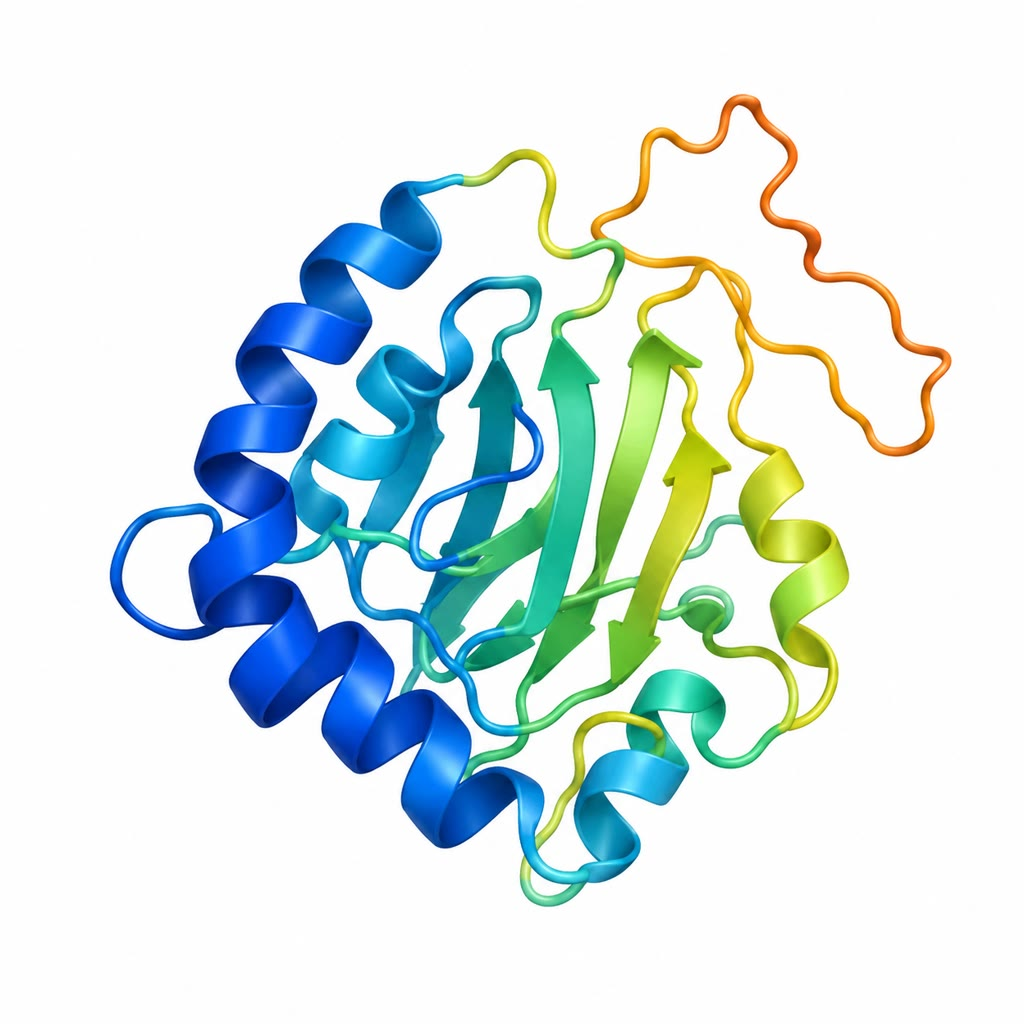
\includegraphics[width=0.36\linewidth]{images/book5/ai/b5-05-alphafold.jpg}\hspace{0.04\linewidth}
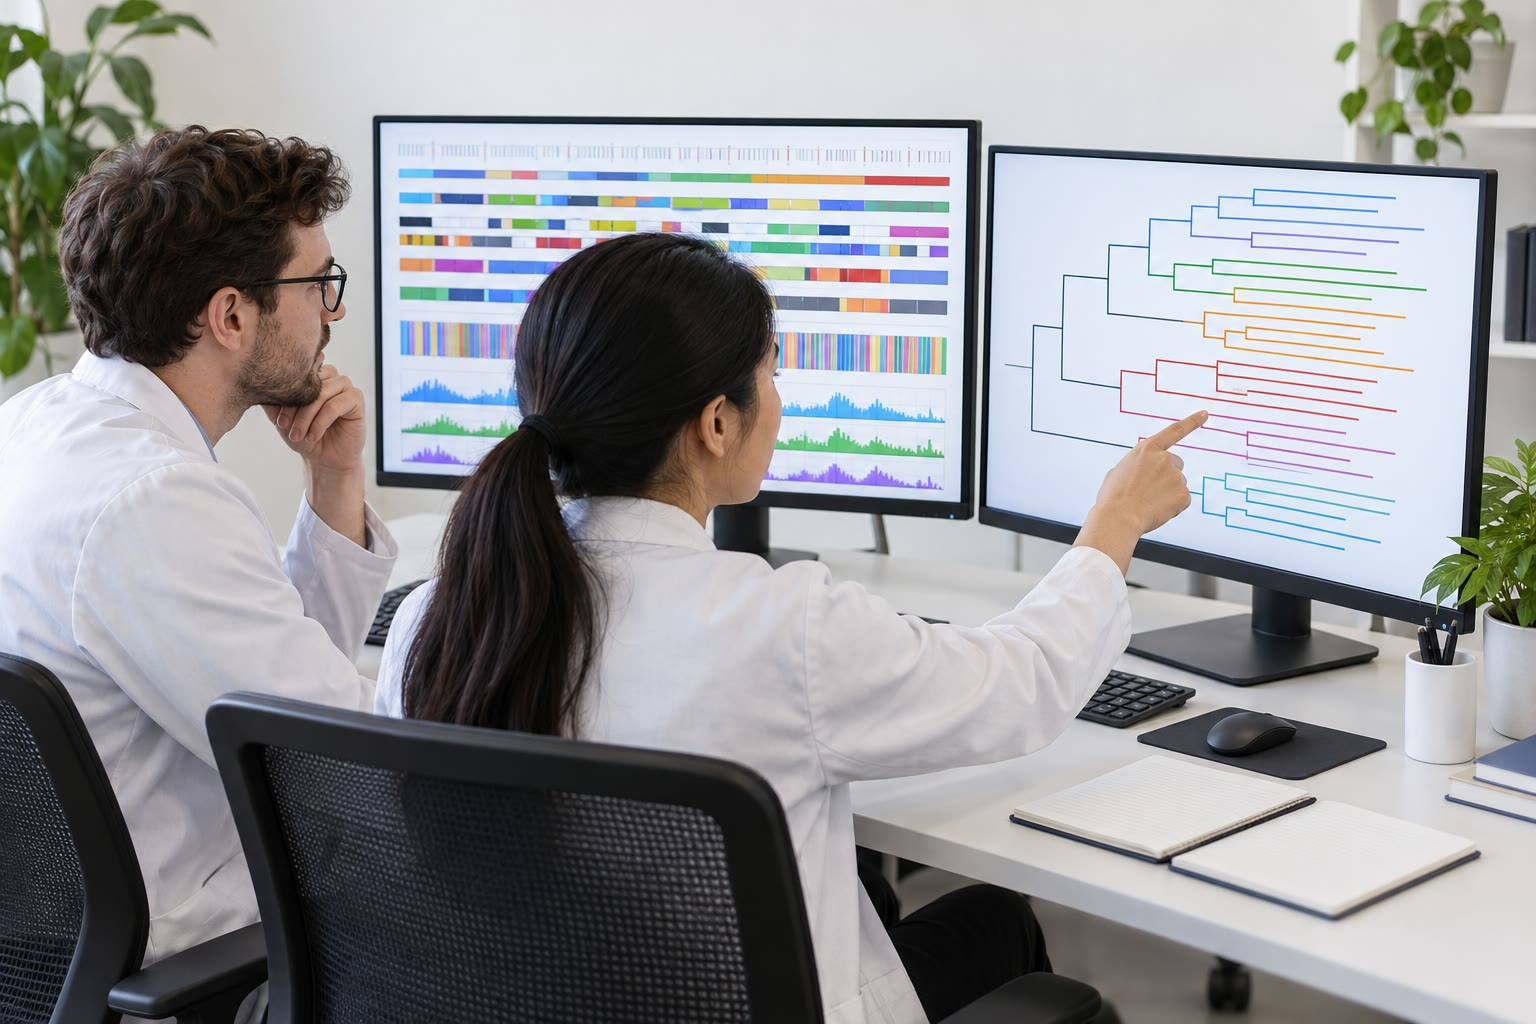
\includegraphics[width=0.54\linewidth]{images/book5/ai/b5-05-bioinformatics-lab.jpg}

{\small Kiri: sebuah struktur protein ramalan, yang diwarnai menurut keyakinan
modelnya dari tinggi (biru) sampai rendah (jingga) pada sebuah lengkung tak
teratur. Kanan: sebuah kantor bioinformatika --- peramban genom dan pohon di
layarnya, dan tanpa satu pun meja basah.}
\end{omfigure}

\begin{remark}[Batas penyimpulan]\label{rem:b3:bioinformatics:limits}
Sebagian besar \omterm{def:b3:genomics:assembly}{anotasi} fungsi di dalam pangkalan data tak pernah diuji;
semuanya dipindahkan dari sebuah homolog, yang sendirinya dianotasi lewat
pemindahan. Galatnya merambat dan berlipat ganda, dan \omterm{def:b3:genomics:assembly}{anotasi} yang keliru pada
protein yang banyak kaitannya dapat menulari satu famili utuh. Penawarnya
adalah penawar di atas: bedakanlah ortologi dari homologi, bacalah
\omterm{def:b3:bioinformatics:alignment}{penjajarannya}, carilah residu katalitiknya, dan ingatlah bahwa ``protein
hipotetis'' adalah label jujur yang masih pantas disandang sepertiga gen di
dalam sebagian besar genom.
\end{remark}

\section{Latihan}

\begin{exercise}[$\star$]\label{exo:b3:bioinformatics:1}
Definisikanlah \omterm{def:b3:bioinformatics:alignment}{penjajaran global} dan \omterm{def:b3:bioinformatics:alignment}{penjajaran lokal} lalu berikanlah satu
keadaan biologis yang menuntut masing-masing.
\end{exercise}

\begin{exercise}[$\star$]\label{exo:b3:bioinformatics:2}
Isilah tabel Needleman--Wunsch bagi AGC terhadap AAC dengan kecocokan $+1$,
ketakcocokan $-1$, celah $-1$, lalu berikan \omterm{def:b3:bioinformatics:alignment}{penjajaran} dan skor optimumnya.
\end{exercise}

\begin{exercise}[$\star$]\label{exo:b3:bioinformatics:3}
Pada BLOSUM62, triptofan--triptofan berskor $+11$ dan leusina--leusina
$+4$. Jelaskanlah dari rumus log-ods mengapa keidentikan residu yang lebih
langka bernilai lebih tinggi.
\end{exercise}

\begin{exercise}[$\star$]\label{exo:b3:bioinformatics:4}
Apa itu nilai-E? Sebuah penelusuran memberi kecocokan dengan $E = 3$. Apa arti
angka itu, dan apakah kecocokannya sebuah homolog?
\end{exercise}

\begin{exercise}[$\star\star$]\label{exo:b3:bioinformatics:5}
Sebuah kueri berisi \num{400} residu ditelusurkan pada $2\times 10^{11}$
residu. Hitunglah nilai-E kecocokan dengan \omterm{thm:b3:bioinformatics:evalue}{skor bit} $45$, $55$, dan
$65$. \omterm{thm:b3:bioinformatics:evalue}{Skor bit} berapa yang memberi $E = 10^{-3}$? Bagaimana jawabannya berubah
bila kuerinya sepanjang \num{40} residu?
\end{exercise}

\begin{exercise}[$\star\star$]\label{exo:b3:bioinformatics:6}
Hitunglah \omterm{def:b3:bioinformatics:motif}{kandungan informasi} sebuah \omterm{def:b3:bioinformatics:motif}{motif} yang keempat kedudukannya
berfrekuensi basa (A, C, G, T) sebesar $(1,0,0,0)$, $(0.5,0,0.5,0)$,
$(0.25,0.25,0.25,0.25)$, dan $(0.7,0.1,0.1,0.1)$. Berapa kecocokan kebetulan
yang dimilikinya di dalam genom \qty{4.6}{Mb}?
\end{exercise}

\begin{exercise}[$\star\star$]\label{exo:b3:bioinformatics:7}
Jelaskanlah mengapa \omterm{def:b3:bioinformatics:alignment}{denda celah} afin lebih masuk akal daripada denda linear,
dan mengapa denda pembukaan celah yang sangat tinggi maupun yang sangat rendah
sama-sama memberi \omterm{def:b3:bioinformatics:alignment}{penjajaran} yang buruk.
\end{exercise}

\begin{exercise}[$\star\star$]\label{exo:b3:bioinformatics:8}
Sebuah penelusuran \omterm{def:b3:bioinformatics:blast}{BLAST} atas sebuah protein manusia pada pangkalan data lalat
memberi kecocokan terbaik dengan $E = 10^{-30}$ yang meliputi residu 50--180
kuerinya yang berisi \num{600} residu. Apakah protein lalat itu \omterm{def:b3:genomics:comparative}{ortolog} protein
manusia tersebut? Uji lanjutan apa yang akan Anda kerjakan?
\end{exercise}

\begin{exercise}[$\star\star$]\label{exo:b3:bioinformatics:9}
Mengapa metode \omterm{def:b3:bioinformatics:msa}{profil} mendeteksi homolog yang terlewat \omterm{def:b3:bioinformatics:alignment}{penjajaran}
berpasangan? Berikanlah sebuah contoh pola lajur yang tertangkap \omterm{def:b3:bioinformatics:msa}{profil}
tetapi tak tertangkap satu urutan tunggal.
\end{exercise}

\begin{exercise}[$\star\star\star$]\label{exo:b3:bioinformatics:10}
Tunjukkanlah bahwa di bawah skema pemberian skor yang \omterm{prop:b3:bioinformatics:logodds}{harapan skornya} positif,
\omterm{def:b3:bioinformatics:alignment}{penjajaran lokal} Smith--Waterman dua urutan acak yang panjang memiliki skor
yang tumbuh lurus dengan panjangnya, lalu jelaskan mengapa hal itu membuat
teori nilai-E gagal. Apa yang tersirat dari hal itu bagi \omterm{def:b3:bioinformatics:alignment}{penjajaran} DNA dengan
kecocokan $+1$ dan ketakcocokan $-1$ pada kandungan GC \qty{60}{\%}?
\end{exercise}

\begin{exercise}[$\star\star\star$]\label{exo:b3:bioinformatics:11}
Tabel Needleman--Wunsch menuntut $mn$ sel ingatan; bagi dua kromosom
\qty{100}{Mb} jumlahnya $10^{16}$. Uraikanlah dua gagasan yang dipakai
penjajar genom untuk menghindarinya (\omterm{def:b3:bioinformatics:blast}{benih} dan perangkaian; pemitaan), dan apa
yang dikorbankan masing-masing.
\end{exercise}

\begin{exercise}[$\star\star\star$]\label{exo:b3:bioinformatics:12}
Sebuah HMM pencari gen bagi bakteri memiliki keadaan bagi ketiga kedudukan
kodonnya dan bagi DNA tak penyandi. Jelaskanlah bagaimana modelnya dapat
membedakan urutan penyandi dari yang tak penyandi tanpa keterangan kodon henti
sama sekali (tinjaulah pemakaian kodonnya), dan mengapa pendekatan yang sama
jauh lebih sukar pada genom manusia.
\end{exercise}

\section{Soal: Sebuah Urutan dari Laut Dalam}

\begin{problem}[{Soal akhir pekan --- sebuah protein tak dikenal yang
dijajarkan dengan tangan, ditelusurkan pada pangkalan data lalu dihitung
kebermaknaannya, motif pengaturnya ditimbang dalam bit, dan gennya diperiksa
terhadap statistika kerangka baca terbuka acak, berakhir pada nilai-E
kecocokan terbaiknya, bit yang dibutuhkan sebuah tapak, dan panjang yang harus
dimiliki sebuah kerangka baca agar dipercaya}]
\label{pb:b3:bioinformatics:1}
Data: sebuah protein berisi \num{300} residu dari anelida laut dalam.
Pangkalan data protein: $1.2\times 10^{11}$ residu. Genom cacingnya:
\qty{1.6}{Gb}, \qty{38}{\%} GC. Pemberian skor bagi \omterm{def:b3:bioinformatics:alignment}{penjajaran} dengan tangan:
kecocokan $+1$, ketakcocokan $-1$, celah $-1$. \omterm{thm:b3:bioinformatics:evalue}{Skor bit} kecocokan \omterm{def:b3:bioinformatics:blast}{BLAST}
terbaiknya: $92$; kecocokan kesepuluhnya: $38$.

\medskip
\noindent\textbf{Bagian I --- Dengan tangan.}
\begin{enumerate}
  \item Jajarkanlah peptida KQT dan KAQT dengan rekurensi
        Needleman--Wunsch: tulislah tabelnya lalu berikan \omterm{def:b3:bioinformatics:alignment}{penjajaran} dan
        skor optimumnya.
  \item Ulangilah dengan Smith--Waterman (lokal) bagi GATCAT terhadap ACAT:
        carilah \omterm{def:b3:bioinformatics:alignment}{penjajaran lokal} terbaiknya dan skornya.
  \item Berapa pembaruan sel yang dibutuhkan \omterm{def:b3:bioinformatics:alignment}{penjajaran global} protein
        berisi \num{300} residu itu terhadap protein berisi \num{450}
        residu? Terhadap seluruh pangkalan datanya?
  \item Bila sebuah komputer melakukan $10^{9}$ pembaruan tiap detik, berapa
        lama \omterm{def:b3:bioinformatics:alignment}{penjajaran} pangkalan data penuh pertanyaan 3 memakan waktu?
        Mengapa \omterm{def:b3:bioinformatics:blast}{BLAST} dipakai sebagai gantinya?
  \item Skor keidentikan BLOSUM62 adalah $+4$ bagi alanina ($p_{A} =
        0.074$) dan $+11$ bagi triptofan ($p_{W} = 0.013$). Dengan
        $\lambda = 0.347$ (satuan setengah bit), hitunglah frekuensi
        sasaran $q_{AA}$ dan $q_{WW}$, serta nisbah $q/p^{2}$ bagi
        masing-masing. Tafsirkanlah.
  \item Dua protein berbagi \qty{24}{\%} keidentikan sepanjang $250$ residu.
        Katakanlah mengapa keidentikan sendirian tak dapat memutuskan
        homologi di sini dan apa yang dapat memutuskannya.
\end{enumerate}

\medskip
\noindent\textbf{Bagian II --- Penelusurannya.}
\begin{enumerate}[resume]
  \item Hitunglah $mn$ bagi kuerinya terhadap pangkalan datanya, dan
        $\log_{2}(mn)$.
  \item Hitunglah nilai-E kecocokan terbaiknya ($S' = 92$) dan kecocokan
        kesepuluhnya ($S' = 38$).
  \item \omterm{thm:b3:bioinformatics:evalue}{Skor bit} berapa yang bersesuaian dengan $E = 10^{-3}$ bagi
        penelusuran ini? Dengan $E = 1$?
  \item Kecocokan terbaik yang sama ditemukan ketika pangkalan datanya telah
        tumbuh menjadi $1.2\times 10^{12}$ residu. Berapa nilai-E-nya?
  \item Kecocokan kesepuluhnya menjajarkan residu 200--260 kuerinya dengan
        keidentikan \qty{40}{\%} sepanjang $60$ residu. Dengan nilai-E-nya,
        katakanlah apakah hal itu menjadi bukti homologi, dan apa yang dapat
        ditambahkan penelusuran \omterm{def:b3:bioinformatics:msa}{profil}.
  \item Kecocokan terbaiknya adalah sebuah kinase manusia, yang terjajar
        sepanjang residu 10--290. Kecocokan terbaiknya di dalam proteom
        cacing itu adalah kuerinya. Apa yang ditegakkan uji timbal balik ini,
        dan apa yang tidak?
\end{enumerate}

\medskip
\noindent\textbf{Bagian III --- Sebuah \omterm{def:b3:bioinformatics:motif}{motif}.}
\begin{enumerate}[resume]
  \item Di hulu gennya terletak sebuah calon tapak faktor transkripsi
        berkedudukan delapan dengan \omterm{def:b3:bioinformatics:motif}{kandungan informasi}
        $2, 2, 1.6, 2, 0.8, 1.2, 0.4, 0.3$ bit. Berapa $R$ totalnya?
  \item Berapa kecocokan kebetulan yang dimiliki \omterm{def:b3:bioinformatics:motif}{motif} itu di dalam genom
        \qty{1.6}{Gb} (kedua untainya, $3.2\times 10^{9}$
        kedudukan)?
  \item Faktornya mengatur sekitar $200$ gen. Berapa bit yang dibutuhkan
        sebuah \omterm{def:b3:bioinformatics:motif}{motif} untuk menentukan $200$ tapak sendirian di dalam genom ini?
  \item Berapa banyak kekurangannya yang dapat dipasok sebuah \omterm{def:b3:bioinformatics:motif}{motif} kedua
        yang bersebelahan dan berisi $8$ bit, bila keduanya harus muncul
        bersama di dalam jarak yang tetap?
  \item Sebuah kedudukan berfrekuensi $(0.5, 0.5, 0, 0)$ bagi (A, C, G,
        T): hitunglah entropinya dan \omterm{def:b3:bioinformatics:motif}{kandungan informasinya}.
  \item Jelaskanlah, dengan argumen informasi itu, mengapa faktor
        transkripsi bakteri lazimnya memiliki tapak yang lebih panjang dan
        lebih lestari daripada faktor eukariot.
\end{enumerate}

\medskip
\noindent\textbf{Bagian IV --- Gennya sendiri.}
\begin{enumerate}[resume]
  \item Di dalam DNA acak yang komposisi basanya seragam, berapa
        peluang sebuah kodon menjadi kodon henti? Berapa harapan
        cacah kodon sebelum sebuah kodon henti muncul (sebaran
        geometrik)?
  \item Genom cacingnya \qty{38}{\%} GC. Hitunglah ulang peluang
        bahwa sebuah kodon acak adalah kodon henti (TAA, TAG, TGA) dengan
        frekuensi basa yang sesungguhnya, dan harapan panjang kerangka
        bacanya. Ke arah mana kandungan GC yang rendah mendorong pencarian gen?
  \item Berapa peluang bahwa sebuah kerangka baca terbuka acak sedikitnya
        sepanjang $100$ kodon? Sedikitnya $300$?
  \item Di dalam genom \qty{1.6}{Gb} itu, enam kerangka pada dua untai
        memberi sekitar $3.2\times 10^{9}$ awalan kodon. Berapa kerangka baca
        terbuka acak sepanjang sedikitnya $100$ kodon yang diharapkan? Berapa
        yang sedikitnya $300$?
  \item Jelaskanlah mengapa ``kerangka baca terbuka yang lebih panjang
        daripada $100$ kodon'' menjadi pencari gen yang berguna pada sebuah
        bakteri tetapi tidak pada genom ini, dan apa yang dipakai pencari gen
        eukariot sebagai gantinya.
  \item Gen cacing itu memiliki enam ekson yang rata-rata \qty{150}{bp}.
        Jelaskanlah bagaimana \omterm{def:b3:genomics:ngs}{bacaan} pengurutan RNA menguraikan struktur
        eksonnya yang ditinggalkan taksa oleh urutan genom saja.
  \item Ringkaskanlah: nilai-E kecocokan terbaiknya (pertanyaan~8), bit
        yang dibutuhkan untuk menentukan $200$ tapak (pertanyaan~15), dan
        harapan cacah kerangka baca acak sepanjang $300$ kodon di dalam
        genomnya (pertanyaan~22).
\end{enumerate}
\end{problem}
